\documentclass[xcolor=dvipsnames,10pt]{beamer}

\beamersetaveragebackground{blue!10}

\mode<presentation>
{
     \usetheme{Warsaw}
}

\usepackage{polski}
\RequirePackage[utf8]{inputenc}

\author{Joanna Kotuła, Aleksandra Mogielska}
\institute[...]{Wydział Matematyki, Informatyki i Mechaniki\\
Uniwersytet Warszawski}

\subject{...}

\title[Intuicyjny język wyszukiwania TQL (Tablets Query Language)]{\bf  Intuicyjny język wyszukiwania TQL \\
Tablets Query Language}
%\subtitle{...}

\date{\today}


\begin{document}
\begin{frame}
     \titlepage
\end{frame}

\begin{frame}
     \frametitle{Spis treści}
     \tableofcontents
\end{frame}
% \begin{frame}
%      \frametitle{Aplikacja wykorzystująca translator}
%    
% \begin{itemize}
% \item umożliwa użytkownikowi wprowadzenie zapytania jako tekstu lub za pomocą graficznego interfejsu
% \item odpowiednio wyświetla zwracanego XML-a, pokazując wyszukiwane sekwencje
% \end{itemize}
% 
% \end{frame}
% 
\chapter*{Wprowadzenie}
\addcontentsline{toc}{chapter}{Wprowadzenie}
%  \begin{figure}
%   \centering
% \includegraphics[width=340px]{./diagramy/poco.pdf}
%   \caption{Zarysowanie problemu}
%  \end{figure}
\begin{figure}[h]
 \centering
 \includegraphics[width=400px]{../diagramy/poco.pdf}
 % poco.pdf: 596x842 pixel, 72dpi, 21.03x29.70 cm, bb=0 0 596 842
 \caption{Przedstawienie problemu}
 \label{fig:poco}
\end{figure}

 
 
Niniejsza praca dotyczy problemu przetwarzania baz danych tabliczek sumeryjskich przez osoby nieznające specyficznych dla baz danych języków zapytań.


Istnieje wiele baz danych zawierających teksty odczytane z tabliczek sumeryjskich (najbardziej znana - CDLI zawiera ich prawie 225 tys.). Sumerolodzy zajmują się badaniem i przetwarzaniem tych tekstów, jednak wyszukiwanie interesujących ich tabliczek jest dosyć niewygodne. Wynika to przede wszystkim z nieznajomości specyficznych dla baz danych języków zapytań. 
Większość serwisów internetowych udostępnia formularze ułatwiające wprowadzanie kryteriów wyszukiwania, jednakże mają one ograniczone możliwości (nie pozwalają na skomplikowane konstrukcje). Dlatego istnieje potrzeba stworzenia narzędzia, które będzie łączyło w sobie jak największą siłę wyrazu i łatwość użycia przez osoby znające jedynie dziedzinę problemu. Celem projektu przedstawionego w niniejszej pracy jest zaprojektowanie i implementacja języka Tablets Query Language (TQL) spełniającego powyższe wymagania. 

TQL jest podstawą do tworzenia podobnych języków wyszukiwań dostosowanych do potrzeb innych grup ludzi, np. językoznawców.
Większość programów ułatwiających tworzenie zapytań jest skomplikowana, daje ograniczone możliwości lub jest przystosowana głównie do przetwarzania danych liczbowych. Tablets Query Language rozwiązuje te problemy: jest prosty i intuicyjny, przystosowany głównie do tekstów, minimalnie zmniejsza siłę wyrazu oraz łatwo go rozbudowywać. 

%Język TQL jest nakładką na inne języki (m.in. SQL). 
Zgodnie z paradygmatem języków dziedzinowych (Domain Specific Languages, DSL) TQL jest nakładką na inne języki zapytań (np. SQL).
% TQL jest jednym z języków dziedzinowych (Domain Specific Languages, DSL). 
W związku z tym dla każdego sposobu reprezentacji danych należy skonstruować translator, 
którego zadaniem będzie przetłumaczenie zapytania. 
% Dla każdego z nich, w zależności od reprezentacji danych, należy skonstruować translator, 
% którego zadaniem będzie przetłumaczenie zapytania. 
W ramach niniejszej pracy przedstawione zostaną dwa przykładowe translatory.


Przy implementacji języka TQL zastosowałyśmy podejście polegające na tzw. preprocessingu - wzorzec Preprocessor \cite{mernik}.
W naszym przypadku polega to na przetłumaczeniu zapytania w języku TQL na zapytanie w innym, istniejącym już języku zapytań wyższego poziomu,
a następnie skorzystaniu z przetłumaczonego w ten sposób zapytania. W tej części pracy przedstawimy sposób zaimplementowania programu tłumaczącego.

Jednym z głównych założeń języka TQL, szczególnie ważnym z punktu widzenia implementacji, jest niezależność od struktury danych.
W związku z tym istotną cechą programu tłumaczącego zapytania w TQL (translatora) jest możliwość dostosowania  
go do współpracy z różnymi bazami danych.
%Jednym z głównych wymagań postawionych przed translatorem, żeby można było podłączyć różne bazy danych.
 Wynikiem tego jest podział translatora na 2 rodzaje modułów (rysunek \ref{moduly}):
\begin{enumerate}
 \item \textbf{Podstawowe} -- niezależne od struktury danych, zajmujące się głównie parsowaniem i analizą składniową zapytania.
 \item \textbf{Wymienne} -- zależne od struktury danych, tłumaczące zapytanie z TQL na język odpowiedni dla używanej bazy danych
i wywołujące je.
\end{enumerate}

\begin{figure}[h]
 \centering
 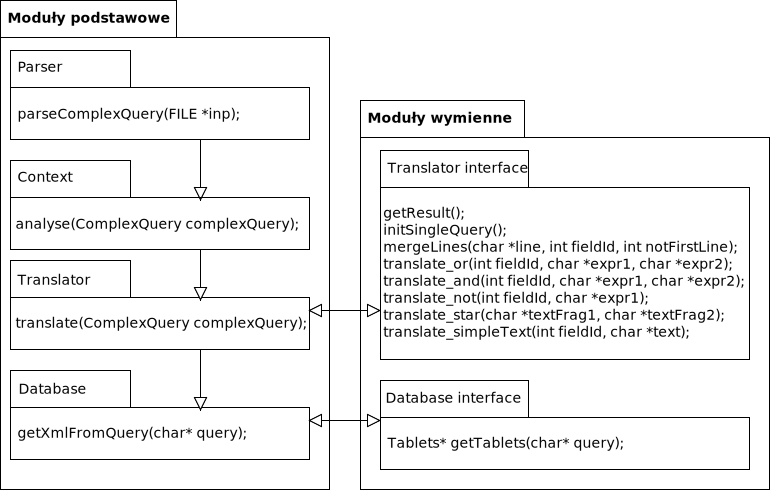
\includegraphics[width=450px]{../diagramy/pakiety.pdf}
 % pakiety.pdf: 585x300 pixel, 72dpi, 20.64x10.58 cm, bb=0 0 585 300
 \caption{Podział programu na moduły}
 \label{moduly}
\end{figure}


Na rysunku \ref{struktura_systemu} przedstawiamy ogólnie strukturę systemu, który korzysta z translatora TQL. Taki system, oprócz modułów podstawowych translatora, zawiera bazę tabliczek w dowolnej formie, implemetację modułów wymiennych umożliwiającą korzystanie z tej bazy, oraz interfejs użytkownika - do wprowadzania zapytań i wyświetlania wyników. \\

 W niniejszej pracy prezentujemy dwie prototypowe implementacje translatora, zawierające własne zestawy modułów wymiennych: 
dla bazy PostgreSQL oraz XML.
%TODO: przeformułować (moduły wymienne na poziomie kompilacji)
   Wybór modułów wymiennych odbywa się na poziomie kompilacji. Jest to rozwiązanie najprostsze do zaimplementowania,
  jednak wymaga osobnego programu dla każdego rodzaju bazy danych.

 Stworzony przez nas Makefile domyślnie buduje obie implementacje translatora TQL.
%Bez względu na wybór modułu wymiennego interfejs całego translatora jest taki sam we wszystkich instancjach.

\begin{figure}[h]
 \centering
 \includegraphics[width=450px,bb=0 0 608 517]{../diagramy/struktura2.pdf}
 % struktura.pdf: 608x517 pixel, 72dpi, 21.45x18.24 cm, bb=0 0 608 517
 \caption{Struktura systemu korzystającego z translatora}
 \label{struktura_systemu}
\end{figure}

\chapter{Moduły podstawowe}

W tym rozdziale przedstawimy dokładniej poszczególne moduły podstawowe translatora.

\section{Parser}
Parser został utworzony za pomocą narzędzia BNFC \cite{bnfc}. Na podstawie etykietowanej gramatyki BNF 
narzędzie to tworzy parser oraz szkielet analizatora składni w wybranym języku: C, C++, C\#, F\#, Haskell, Java lub OCaml. 
BNFC tworzy również pliki wejściowe dla generatora leksera (np. Flex) oraz dla generatora parsera (np. Bison). 
Dodatkowym produktem jest dokument w formacie Latex, który zawiera specyfikację zaprojektowanego języka.


Po automatycznym utworzeniu parsera, 
poprawiłyśmy nazwy stałych oznaczających symbole na bardziej intuicyjne.
Następnie
dodałyśmy tablicę symboli,
usunęłyśmy niepotrzebne funkcje z interfejsu
i ogólnie uporządkowałyśmy kod.

Moduł  parsuje zapytanie w języku TQL, tworząc drzewo struktury składniowej, które jest zdefiniowane w pliku pomocniczym Absyn.h.

Główna funkcja tego modułu to \verb|parseComplexQuery(FILE *inp)|. Argumentem jest wskaźnik do pliku zawierającego zapytanie TQL, 
a wynikiem odpowiednie drzewo struktury składniowej.

Na parser składają się następujące pliki:
\begin{itemize}
 \item Parser.cpp
 \item Parser.h
 \item TQL.y % tłumaczony na Parser.c
 \item TQL.l % tłumaczony na Lexer.c
\end{itemize}


\section{Analizator kontekstowy}
Podstawową funkcją w tym module jest \verb|analyse(ComplexQuery complexQuery)|, której argumentem oraz wynikiem jest 
drzewo struktury składniowej zapytania TQL. Funkcja ta
 sprawdza, czy podano prawidłowe nazwy pól, na podstawie których następuje wyszkukiwanie,  %to co jest po lewej w linii zapytania jest nazwą pola.
oraz upraszcza drzewo - z wywołania zapytania (wywołanie \textit{search in}) tworzy zapytanie proste.

Analizator kontekstowy składa się z następujących plików:
\begin{itemize}
 \item Context.cpp
 \item Context.h
\end{itemize}

\section{Translator}
Zadaniem translatora jest przetłumaczenie drzewa składni abstrakcyjnej na zapytanie w docelowym języku.
Składa się z następujących plików:
\begin {itemize}
 \item Translator.cpp
 \item Translator.h
 \item Translator\_interface.h (interfejs modułu translatora zależnego od bazy danych)
 %\item Translator\_config.c (implementacja interfejsu z Translator\_config.h, zależny od wyboru bazy danych itp)
\end {itemize}

Tłumaczenie poszczególnych elementów drzewa zależy od implementacji interfejsu zawartego w pliku Translator\_interface.h. 
Funkcja \verb|translate(ComplexQuery complexQuery)| przechodzi całą strukturę drzewa, wywołując w razie 
potrzeby odpowiednie funkcje z Translator\_interface.
Następnie pobiera przetłumaczone zapytanie za pomocą funkcji getResult() i przekazuje je jako wynik.

\section{Baza}
Moduł bazy jest odpowiedzialny za wywołanie przetłumaczonego zapytania i przekazanie wyniku w określonej formie - jako XML.
Składa się z następujących plików:
\begin {itemize}
 \item Database.cpp
 \item Database.h
 \item Database\_interface.h (interfejs modułu bazy zależnego od bazy danych)
% \item Database\_config.c (implementacja interfejsu z Database\_conf.h, zależny od wyboru bazy danych itp)
\end {itemize}

Główną funkcją w tym module jest \verb|getXmlFromQuery(char *query)|, która
wywołuje funkcję \verb|getTablets(char *query|) z Database\_interface.h, jako parametr podając przetłumaczoną treść zapytania. 
Dostaje w wyniku strukturę danych Tablets, wypełnioną informacjami o wyszukanych tabliczkach.
Następnie na podstawie otrzymanej struktury tworzy dokument XML i przekazuje go jako wynik wywołania zapytania.
\newline
Struktura Tablets zawiera metadane tabliczki, jej treść oraz informację o frazach, na podstawie których tabliczka została znaleziona. 
Poniżej przedstawiamy definicję struktury Tablets:
\begin{verbatim}
typedef struct{    
    char* id;
    char* id_cdli;
    char* publication;
    char* measurements;
    char* year;
    char* provenience;
    char* period;
    char* genre;
    char* subgenre;
    char* collection;
    char* text;
    Tags* tags; // specjalnie oznaczone miejsca w tekscie - frazy wyszukiwania
} Tablet;

typedef struct{
    int size;
    Tablet* tabs;
} Tablets;
\end{verbatim}

% TODO: czy tak jest ok?
Zakładamy, że w bazie danych znajdują się informacje potrzebne do wypełnienia powyższej struktury.
%Wszystkie niezbędne informacje powinny się znajdować w bazie danych.

\section{Pliki pomocnicze}
Definicje struktur danych i funkcji służących do budowy drzewa struktury składniowej (wygenerowane za pomocą BNFC \cite{bnfc}, 
następnie uproszczone):
\begin{itemize}
 \item Absyn.cpp
 \item Absyn.h
\end{itemize}
Tablica symboli:
\begin{itemize}
 \item Symbols.cpp
\item Symbols.h
\end{itemize}
Obsługa błędów:
\begin{itemize}
 \item Err.cpp
\item Err.h
\end{itemize}
Moduł do dzielenia tekstu względem separatora, pobrany z internetu \cite{cexplode}:
\begin{itemize}
 \item Cexplode.cpp
 \item Cexplode.h
\end{itemize}


\chapter{Moduły wymienne}
Pliki zależne od wyboru konkretnej bazy danych to:
\begin{itemize}
 \item Translator\_$<$nazwa$>$.cpp - dla modułu translatora
\item Database\_$<$nazwa$>$.cpp - dla modułu bazy
\end{itemize}
Ich interfejsy są wspólne dla wszystkich baz danych.

\subsection{PostgreSQL}

\begin{frame}
 \frametitle{Diagram encji}
 \includegraphics[width=100mm]{../diagramy/diagram-encji-maly.pdf}
\end{frame}

\begin{frame}
 \frametitle{Tłumaczenie zapytań: inicjalizacja}
 \begin{block}{Select}
SELECT t.id, t.id\_cdli, t.publication, t.measurements, t.origin\_date, \\
~~~~~~~p.value as provenience, pd.value as period, \\
~~~~~~~g1.value as genre, g2.value as subgenre, \\
~~~~~~~c.value as collection, t.text 
 \end{block}
\begin{block}{From}
FROM tablet t \\
~~LEFT JOIN provenience p ON p.id=t.provenience\_id \\
~~LEFT JOIN collection c ON c.id=t.collection\_id \\
~~LEFT JOIN genre g1 ON g1.id=t.genre\_id \\
~~LEFT JOIN genre g2 ON g2.id = t.subgenre\_id \\
~~LEFT JOIN period pd ON pd.id = t.period\_id \\
\end{block}

\end{frame}

\begin{frame}
 \frametitle{Tłumaczenie zapytań: zapytania proste}

\end{frame}

\begin{frame}
 \frametitle{Tłumaczenie zapytań: treść tabliczki}

% \begin{block}{From}
% 
% INNER JOIN ( \\
% 
% ) AS sequence ON sequence.id\_tab = t.id \\
%  \end{block}

 \begin{block}{wynikowe zapytanie o treść tablczki}
\begin{scriptsize}
SELECT \\
~~id\_tab, \\
~~CAST(array\_accum(nodes) as TEXT) as nodes,\\
~~COUNT(DISTINCT id\_seq) AS seq,\\
~~$<$id\_seq$>$ AS id\_seq\\
FROM (\\
~~SELECT\\
~~~~t1.node1\_id \% 1000000 AS id\_tab,\\
~~~~’\{’ $||$ t1.node1\_id $||$ ’,’ $||$ t$<$dl\_sekw$>$.node2\_id $||$ ’\}’ AS nodes,\\
~~~~1 AS id\_seq\\
~~FROM\\
~~~~readings t1\\
~~~~LEFT JOIN readings t2 ON (t2.node1 = t1.node2)\\
~~~~LEFT JOIN $<$nazwa\_tabeli$>$ t3 ON (t3.node1 = t2.node2)\\
~~~~...\\
~~~~LEFT JOIN $<$nazwa\_tabeli$>$ t$<$dl\_sekw$>$ ON (t$<$dl\_sekw$>$.node1 = t$<$dl\_sekw-1$>$.node2)\\
~~WHERE\\
~~~~t1.value LIKE ’$<$sekw[1]$>$’\\
~~~AND\\
~~~~t2.value LIKE ’$<$sekw[2]$>$’\\
~~~AND\\
~~~~t3.value LIKE ’$<$sekw[3]$>$’\\
~~~AND\\
~~~~...\\
~~~AND\\
~~~~t$<$dl\_sekw$>$.value LIKE ’$<$sekw[$<$dl\_sekw$>$]$>$’\\
) AS a
GROUP BY id\_tab

\end{scriptsize}
 \end{block}


\end{frame}


\subsection{XML}
\begin{frame}
 \frametitle{Schemat}

\end{frame}

% \section{Co zrobiłyśmy, co planujemy}
% %  Problemy (?) planowane optymalizacje (coś ciekawego na pewno musi 
% % być), featury (planowane)
% 
% 
% \begin{frame}
%      \frametitle{Do tej pory}
%      
% \begin{itemize}
% \item przykładowa baza relacyjna (Postgres)
% \item gotowy parser i analizator składniowy
% \item moduł translatora i moduł konfiguracyjny dla bazy relacyjnej
% \item moduł bazy: połączenie z bazą, wykonywanie zapytań i zwracanie XML-a -- jeszcze bez zaznaczonych sekwencji wyszukiwania
% \end{itemize}
% 
% 
% \end{frame}
% 
% \begin{frame}
%      \frametitle{Plany}
%      
% \begin{itemize}
% \item zaznaczanie w XML-u z tabliczkami wyszukiwanych sekwencji
% \item interfejs graficzny -- do wprowadzania zapytań i wyświetlania wyników
% \item moduły konfiguracyjne do innej bazy danych
% \item optymalizacje zapytań (obowiązkowo dla negacji)
% \item tłumaczenie odczyty $\leftrightarrow$  kliny i wyszukiwanie po klinach
% \end{itemize}
% \end{frame}


% 
%\section{Pokaz działania}

%\begin{frame}
%     \frametitle{Pokaz działania}
%\end{frame}


\end{document}




